\documentclass[11pt,a4paper]{article}

\usepackage{../ve230}

\author{\href{liuyh615@sjtu.edu.cn}{Yihao Liu} (515370910207)}
\semester{Summer}
\year{2019}
\subtitle{Homework}
\subtitlenumber{1}
\blockinfo{}

\usetikzlibrary{positioning}

\begin{document}

\maketitle

\subsection{2-11}
\begin{center}
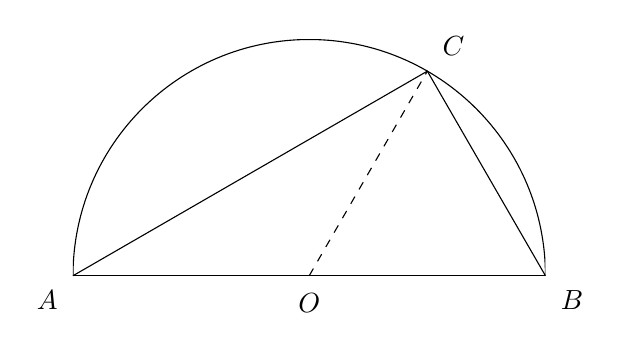
\begin{tikzpicture}[baseline=(current bounding box.north),scale=2]
\begin{scope}
    \clip (-1.5,0) rectangle (1.5,1.5);
    \draw (0,0) circle(1.5);
    \draw (-1.5,0) -- (1.5,0);
\end{scope}
\node[below left= 1mm of {(-1.5,0)}] {$A$};
\node[below= 1mm of {(0,0)}] {$O$};
\node[below right= 1mm of {(1.5,0)}] {$B$};
\node[above right= 1mm of {(60:1.5)}] {$C$};
\draw (-1.5,0) -- (60:1.5) -- (1.5,0);
\draw[dashed] (0,0) -- (60:1.5);
\end{tikzpicture}
\end{center}

Since $OA=OB=OC$, we know $\angle OAC=\angle OCA$ and $\angle OBC=\angle OCB$. And since $ABC$ is an triangle, $\angle OAC+\angle OBC+\angle ACB=\pi$, we can simply find that $\angle ACB=\pi/2$, so that an angle inscribed in a semicircle is a right angle.

\subsection{2-17}
\begin{enumerate}[label=\alph*)]
\item 
$$|\mathbf{E}|=|\mathbf{a_R}(25/R^2)|=|\mathbf{a_R}|\cdot\frac{25}{3^2+4^2+5^2}=\frac{1}{2}.$$
$$E_x=|\mathbf{E}|\cdot\frac{x}{R}=\frac{1}{2}\cdot\frac{-3}{\sqrt{3^2+4^2+5^2}}=-\frac{3\sqrt{2}}{20}.$$
\item
$$\cos\theta=\frac{\mathbf{E}\cdot\mathbf{B}}{|\mathbf{E}||\mathbf{B}|}=\frac{-3\cdot2+4\cdot-2-5\cdot1}{\sqrt{3^2+4^2+5^2}\cdot\sqrt{2^2+2^2+1^1}}=-\frac{19\sqrt{2}}{30},$$
$$\theta=\arccos-\frac{19\sqrt{2}}{30}\approx \SI{2.681}{\radian}.$$
\end{enumerate}

\subsection{2-21}
$$\int_{P_1}^{P_2}\mathbf{E}\cdot d\mathbf{l}=\int_{P_1}^{P_2}(\mathbf{a_x}y+\mathbf{a_y}x)(\mathbf{a_x}dx+\mathbf{a_y}dy)=\int_{P_1}^{P_2}(ydx+xdy)$$
\begin{enumerate}[label=\alph*)]
\item
$$\int_{P_1}^{P_2}\mathbf{E}\cdot d\mathbf{l}=\int_{P_1}^{P_2}(y\cdot4ydy+2y^2\cdot dy)=\int_1^2 6y^2dy=14.$$
\item
$$x=6y-4,$$
$$\int_{P_1}^{P_2}\mathbf{E}\cdot d\mathbf{l}=\int_{P_1}^{P_2}[y\cdot6dy+(6y-4)\cdot dy]=\int_1^2 (12y-4)dy=14.$$
\end{enumerate}

\subsection{2-26}
\begin{enumerate}[label=\alph*)]
\item
$$\nabla\cdot f_1(\mathbf{R})=\frac{1}{R^2}\cdot\frac{\partial}{\partial R}(R^n\cdot R^2)=(n+2)R^{n-1}.$$
\item
$$\nabla\cdot f_2(\mathbf{R})=\frac{1}{R^2}\cdot\frac{\partial}{\partial R}(k/R^2\cdot R^2)=0.$$
\end{enumerate}

\subsection{2-29}
$$\nabla\cdot\mathbf{A}=\frac{1}{r}\cdot\frac{\partial}{\partial r}(r^2\cdot r)+\frac{\partial}{\partial z}(2z)=3r+2.$$
$$\int_V\nabla\cdot\mathbf{A}dV=\int_V(3r+2)dV=\int_0^4\int_0^{2\pi}\int_0^5(3r+2)rdrd\theta dz=1200\pi.$$
$$\oint_S\mathbf{A}dS=\int_0^4\int_0^{2\pi}(\mathbf{a_r}r^2)rd\theta dz\mathbf{a_r}+\int_0^{2\pi}\int_0^52z\mathbf{a_z}rdrd\theta\mathbf{a_z}=1000\pi+200\pi=1200\pi.$$
So $$\int_V\nabla\cdot\mathbf{A}dV=\oint_S\mathbf{A}dS.$$

\subsection{2-33}
$$\nabla\cdot(\mathbf{E}\times\mathbf{H})=\frac{\partial}{\partial x}(E_yH_z-E_zH_y)+\frac{\partial}{\partial y}(E_zH_x-E_xH_z)+\frac{\partial}{\partial z}(E_xH_y-E_yH_x),$$
$$\mathbf{H}\cdot(\nabla\times\mathbf{E})=H_x\left(\frac{\partial E_z}{\partial y}-\frac{\partial E_y}{\partial z}\right)+H_y\left(\frac{\partial E_x}{\partial z}-\frac{\partial E_z}{\partial x}\right)+H_z\left(\frac{\partial E_y}{\partial x}-\frac{\partial E_x}{\partial y}\right),$$
$$\mathbf{E}\cdot(\nabla\times\mathbf{H})=E_x\left(\frac{\partial H_z}{\partial y}-\frac{\partial H_y}{\partial z}\right)+E_y\left(\frac{\partial H_x}{\partial z}-\frac{\partial H_z}{\partial x}\right)+E_z\left(\frac{\partial H_y}{\partial x}-\frac{\partial H_x}{\partial y}\right).$$
Since
$$\frac{\partial}{\partial x}AB=A\frac{\partial B}{\partial x}+B\frac{\partial A}{\partial x},$$
we can find that
$$\nabla\cdot(\mathbf{E}\times\mathbf{H})=\mathbf{H}\cdot(\nabla\times\mathbf{E})-\mathbf{E}\cdot(\nabla\times\mathbf{H}).$$

\subsection{2-35}
$$\Delta s_u=R^2\sin\theta\Delta\theta\Delta\phi,$$
\begin{align*}
\oint_{C_u}\mathbf{A}\cdot d\mathbf{l}=&A_\theta\cdot(R,\theta,\phi-\Delta\phi/2)R\Delta\theta-A_\theta\cdot(R,\theta,\phi+\Delta\phi/2)R\Delta\theta+\\
&A_\phi\cdot(R,\theta+\Delta\theta/2,\phi)R\Delta\phi\sin(\theta+\Delta\theta/2)-A_\phi\cdot(R,\theta-\Delta\theta/2,\phi)R\Delta\phi\sin(\theta-\Delta\theta/2)\\
=&-\frac{\partial A_\theta}{\partial\phi}R\Delta\phi\Delta\theta+\frac{\partial A_\phi\sin\theta}{\partial\theta}R\Delta\phi\Delta\theta.
\end{align*}
\begin{align*}
(\nabla\times\mathbf{A})_u&=\lim_{\Delta s_u\to0}\frac{1}{\Delta s_u}\oint_{C_u}\mathbf{A}\cdot d\mathbf{l}=\lim_{\Delta s_u\to0}\frac{1}{R^2\sin\theta\Delta\theta\Delta\phi}\cdot\left(-\frac{\partial A_\theta}{\partial\phi}+\frac{\partial A_\phi\sin\theta}{\partial\theta}\right)R\Delta\phi\Delta\theta\\
&=\frac{1}{R\sin\theta}\cdot\left(-\frac{\partial A_\theta}{\partial\phi}+\frac{\partial A_\phi\sin\theta}{\partial\theta}\right).
\end{align*}
$$$$

\subsection{2-39}
\begin{enumerate}[label=\alph*)]
\item
$$\nabla\times\mathbf{F}=\mathbf{a_x}(c_3+3)+\mathbf{a_y}(c_1-1)+\mathbf{a_z}c_2=\mathbf{0},$$
$$c_1=1,c_2=0,c_3=-3.$$
\item
$$\nabla\cdot\mathbf{F}=1+0+c_4=0,$$
$$c_4=-1.$$
\item
$$\mathbf{F}=-\nabla V=\mathbf{a_x}(x+z)+\mathbf{a_y}(-3z)+\mathbf{a_z}(x-3y-z),$$
$$V=-\frac{1}{2}x^2-xz+3yz+\frac{1}{2}z^2+C.$$
\end{enumerate}

\end{document}


